\documentclass[aspectratio=169]{beamer}

\usepackage[T1]{fontenc}
\usepackage[utf8]{inputenc}
\usepackage{amsmath,amssymb,bm}
\usepackage{booktabs}
\usepackage{tikz}
\usetikzlibrary{arrows.meta,positioning,shapes.geometric,fit}

\usetheme{default}
\usecolortheme{default}
\setbeamertemplate{navigation symbols}{}
\setbeamertemplate{footline}[frame number]
\setbeameroption{hide notes}

\definecolor{DeepNavy}{HTML}{0B1320}
\definecolor{SignalGreen}{HTML}{16A34A}
\definecolor{WarmGold}{HTML}{D97706}
\definecolor{SoftGray}{HTML}{F3F4F6}
\definecolor{Ink}{HTML}{111827}
\definecolor{Muted}{HTML}{4B5563}
\definecolor{Panel}{HTML}{EEF2F7}

\setbeamercolor{title}{fg=DeepNavy}
\setbeamercolor{frametitle}{fg=DeepNavy}
\setbeamercolor{normal text}{fg=Ink,bg=white}
\setbeamercolor{structure}{fg=SignalGreen}
\setbeamercolor{block title}{fg=white,bg=DeepNavy}
\setbeamercolor{block body}{fg=Ink,bg=Panel}
\setbeamerfont{frametitle}{series=\bfseries,size=\large}

\newcommand{\takeaway}[1]{%
  \begin{block}{Main takeaway}
    #1
  \end{block}
}

\newcommand{\dataset}{\mathcal D}
\newcommand{\states}{\mathcal S}
\newcommand{\actions}{\mathcal A}

\title{From Control to Offline Reinforcement Learning}
\subtitle{Learning Better Decisions from Logged Data}
\author{Stephan Mandt}
\institute{}
\date{\today}

\begin{document}

\begin{frame}[plain,noframenumbering]
  \begin{tikzpicture}[remember picture,overlay]
    \fill[DeepNavy] (current page.south west) rectangle (current page.north east);
    \begin{scope}[shift={(current page.south west)}]
      \fill[SignalGreen] (0,0) rectangle (0.18,9);
      \fill[WarmGold] (0.18,0) rectangle (0.25,9);
    \end{scope}
  \end{tikzpicture}

  \vspace*{1.0cm}
  {\color{white}\Huge\bfseries\inserttitle\par}
  \vspace{0.3cm}
  {\color{SoftGray}\Large\insertsubtitle\par}

  \vfill
  {\color{SignalGreen}\insertauthor}
  \hspace{0.6cm}
  {\color{SoftGray!75}\insertdate}
  \note{Open with the thesis: RL is data-driven optimal control. Offline RL is the product-relevant version when interaction is expensive, risky, slow, or constrained.}
\end{frame}

\section{Product Motivation}

\begin{frame}{Predictions Are Not Decisions}
  \centering
  \begin{tabular}{p{0.43\textwidth}p{0.43\textwidth}}
    \toprule
    \textbf{Supervised learning predicts} & \textbf{RL chooses} \\
    \midrule
    Truck arrival time & Which truck to unload next \\
    Unloading duration & Which pit to assign \\
    Grain quality & Which silo to route into \\
    Train delay & How to schedule train loading \\
    \bottomrule
  \end{tabular}

  \vspace{0.5cm}
  \takeaway{Supervised learning predicts what happens next. Reinforcement learning chooses what should happen next.}
  \note{Open with the grain terminal. Prediction is useful, but the product tension starts when the system must choose an action that changes the operation.}
\end{frame}

\begin{frame}{Actions Change the Future}
  \centering
  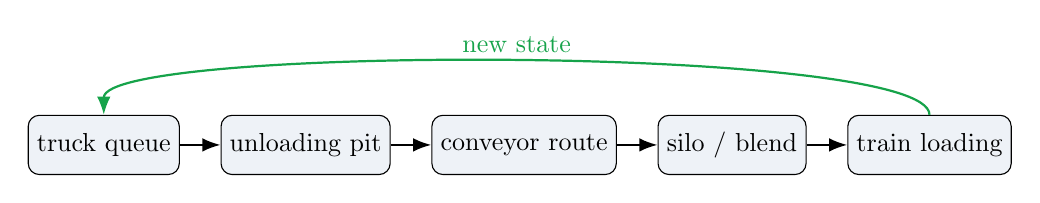
\begin{tikzpicture}[node distance=0.55cm,>=Latex,scale=0.94,transform shape]
    \node[draw,rounded corners,fill=Panel,minimum width=2.0cm,minimum height=0.8cm] (queue) {truck queue};
    \node[draw,rounded corners,fill=Panel,right=of queue,minimum width=2.0cm,minimum height=0.8cm] (pit) {unloading pit};
    \node[draw,rounded corners,fill=Panel,right=of pit,minimum width=2.1cm,minimum height=0.8cm] (route) {conveyor route};
    \node[draw,rounded corners,fill=Panel,right=of route,minimum width=2.0cm,minimum height=0.8cm] (silo) {silo / blend};
    \node[draw,rounded corners,fill=Panel,right=of silo,minimum width=2.0cm,minimum height=0.8cm] (train) {train loading};
    \draw[->,thick] (queue) -- (pit);
    \draw[->,thick] (pit) -- (route);
    \draw[->,thick] (route) -- (silo);
    \draw[->,thick] (silo) -- (train);
    \draw[->,thick,SignalGreen] (train.north) .. controls +(0,0.95) and +(0,0.95) .. node[above]{new state} (queue.north);
  \end{tikzpicture}

  \vspace{0.45cm}
  Choosing a truck, pit, route, or silo changes future queues, storage, blending options, and train schedules.

  \vspace{0.25cm}
  \productbox{In RL, the model does not just observe the data distribution. It helps create the next data distribution.}
  \note{This is the main conceptual gap. Supervised learning assumes a fixed data distribution; a policy changes the states it will see next.}
\end{frame}

\begin{frame}{States, Actions, and Policies}
  \centering
  \begin{tabular}{p{0.22\textwidth}p{0.65\textwidth}}
    \toprule
    \textbf{Object} & \textbf{Grain-terminal example} \\
    \midrule
    state $s_t$ & current queue, silo inventory, grain quality, train progress \\
    action $a_t$ & unload truck, choose pit, route conveyor, assign silo, fill car \\
    policy $\pi(a\mid s)$ & rule or model that chooses actions from states \\
    next state $s_{t+1}$ & the facility after the action has changed it \\
    \bottomrule
  \end{tabular}

  \vspace{0.55cm}
  \takeaway{A decision problem starts with states, actions, and a policy that maps situations to decisions.}
  \note{Define the basic vocabulary before imitation learning uses it. State means the information available at decision time. Action means the decision we control. A policy is the rule or learned model that maps states to actions.}
\end{frame}

\begin{frame}{Why RL Needs More Than Logs}
  \centering
  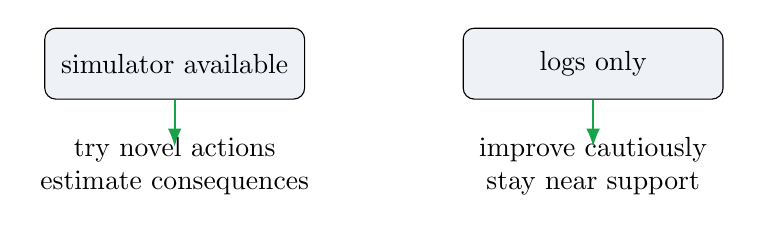
\begin{tikzpicture}[node distance=0.9cm,>=Latex]
    \node[draw,rounded corners,fill=Panel,minimum width=3.3cm,minimum height=0.9cm] (sim) {simulator available};
    \node[draw,rounded corners,fill=Panel,right=2.0cm of sim,minimum width=3.3cm,minimum height=0.9cm] (logs) {logs only};
    \node[below=0.35cm of sim,text width=3.5cm,align=center] {try novel actions\\estimate consequences};
    \node[below=0.35cm of logs,text width=3.5cm,align=center] {improve cautiously\\stay near support};
    \draw[->,thick,SignalGreen] (sim.south) -- ++(0,-0.6);
    \draw[->,thick,SignalGreen] (logs.south) -- ++(0,-0.6);
  \end{tikzpicture}

  \vspace{1.0cm}
  \takeaway{RL is about policy improvement, not just action prediction.}
  \note{This sets up the later offline RL material. If we have a simulator, RL can evaluate counterfactual actions. If we only have logs, offline RL must improve while respecting dataset support.}
\end{frame}

\begin{frame}{The RL Question}
  \Large
  Given logged grain-terminal decisions and delayed outcomes, can we learn a better policy without risky online experimentation?

  \vspace{0.6cm}
  \normalsize
  Logged data:
  \[
    (s_t, a_t, \text{outcome}, s_{t+1})
  \]

  \vspace{0.2cm}
  \productbox{This is the bridge from product operations to imitation learning and the RL formalism.}
  \note{Use this as the transition into imitation learning and then the RL formalism. We now have states, actions, delayed outcomes, and a policy to improve.}
\end{frame}

\section{First Obvious Idea: Imitate Good Operators}

\begin{frame}{Imitation Learning: Turn Decisions Into Supervised Learning}
  \large
  First idea: collect observed behavior and train a policy to predict what the operator would do.

  \vspace{0.12cm}
  \normalsize
  Historical demonstrations come from a \alert{behavior policy} $\pi_b$, e.g. human terminal operators:
  \[
    \dataset = \{(s_t,a_t)\},
    \qquad
    a_t \sim \pi_b(a\mid s_t)
  \]

  \vspace{0.02cm}
  Train $\pi_\theta$ as a supervised action predictor:
  \begin{columns}[T,onlytextwidth]
    \begin{column}{0.48\textwidth}
      \textbf{Continuous actions}\\[-0.1cm]
      {\small steering angle, conveyor speed}
      \[
        \min_\theta\
        \mathbb E_{\dataset}
        \left[\|a-\pi_\theta(s)\|^2\right]
      \]
    \end{column}
    \begin{column}{0.48\textwidth}
      \textbf{Discrete actions}\\[-0.1cm]
      {\small route choice, silo assignment}
      \[
        \min_\theta\
        -\mathbb E_{\dataset}
        \left[\log \pi_\theta(a\mid s)\right]
      \]
    \end{column}
  \end{columns}

  \vspace{0.1cm}
  Attractive because it is fully offline, simple to train, and does not require defining a reward.
  \note{This is the baseline everyone should think of first. We collect states and actions from a behavior policy pi-b, such as human operators, and train a new policy to predict those actions. Continuous controls become regression problems; discrete decisions become classification problems. The attraction is that this looks almost exactly like standard supervised learning.}
\end{frame}

\begin{frame}{Pitfall 1: Averaging Demonstrations Can Fail}
  \begin{columns}[T,onlytextwidth]
    \begin{column}{0.48\textwidth}
      \centering
      \IfFileExists{assets/lane_change_car.jpg}{%
        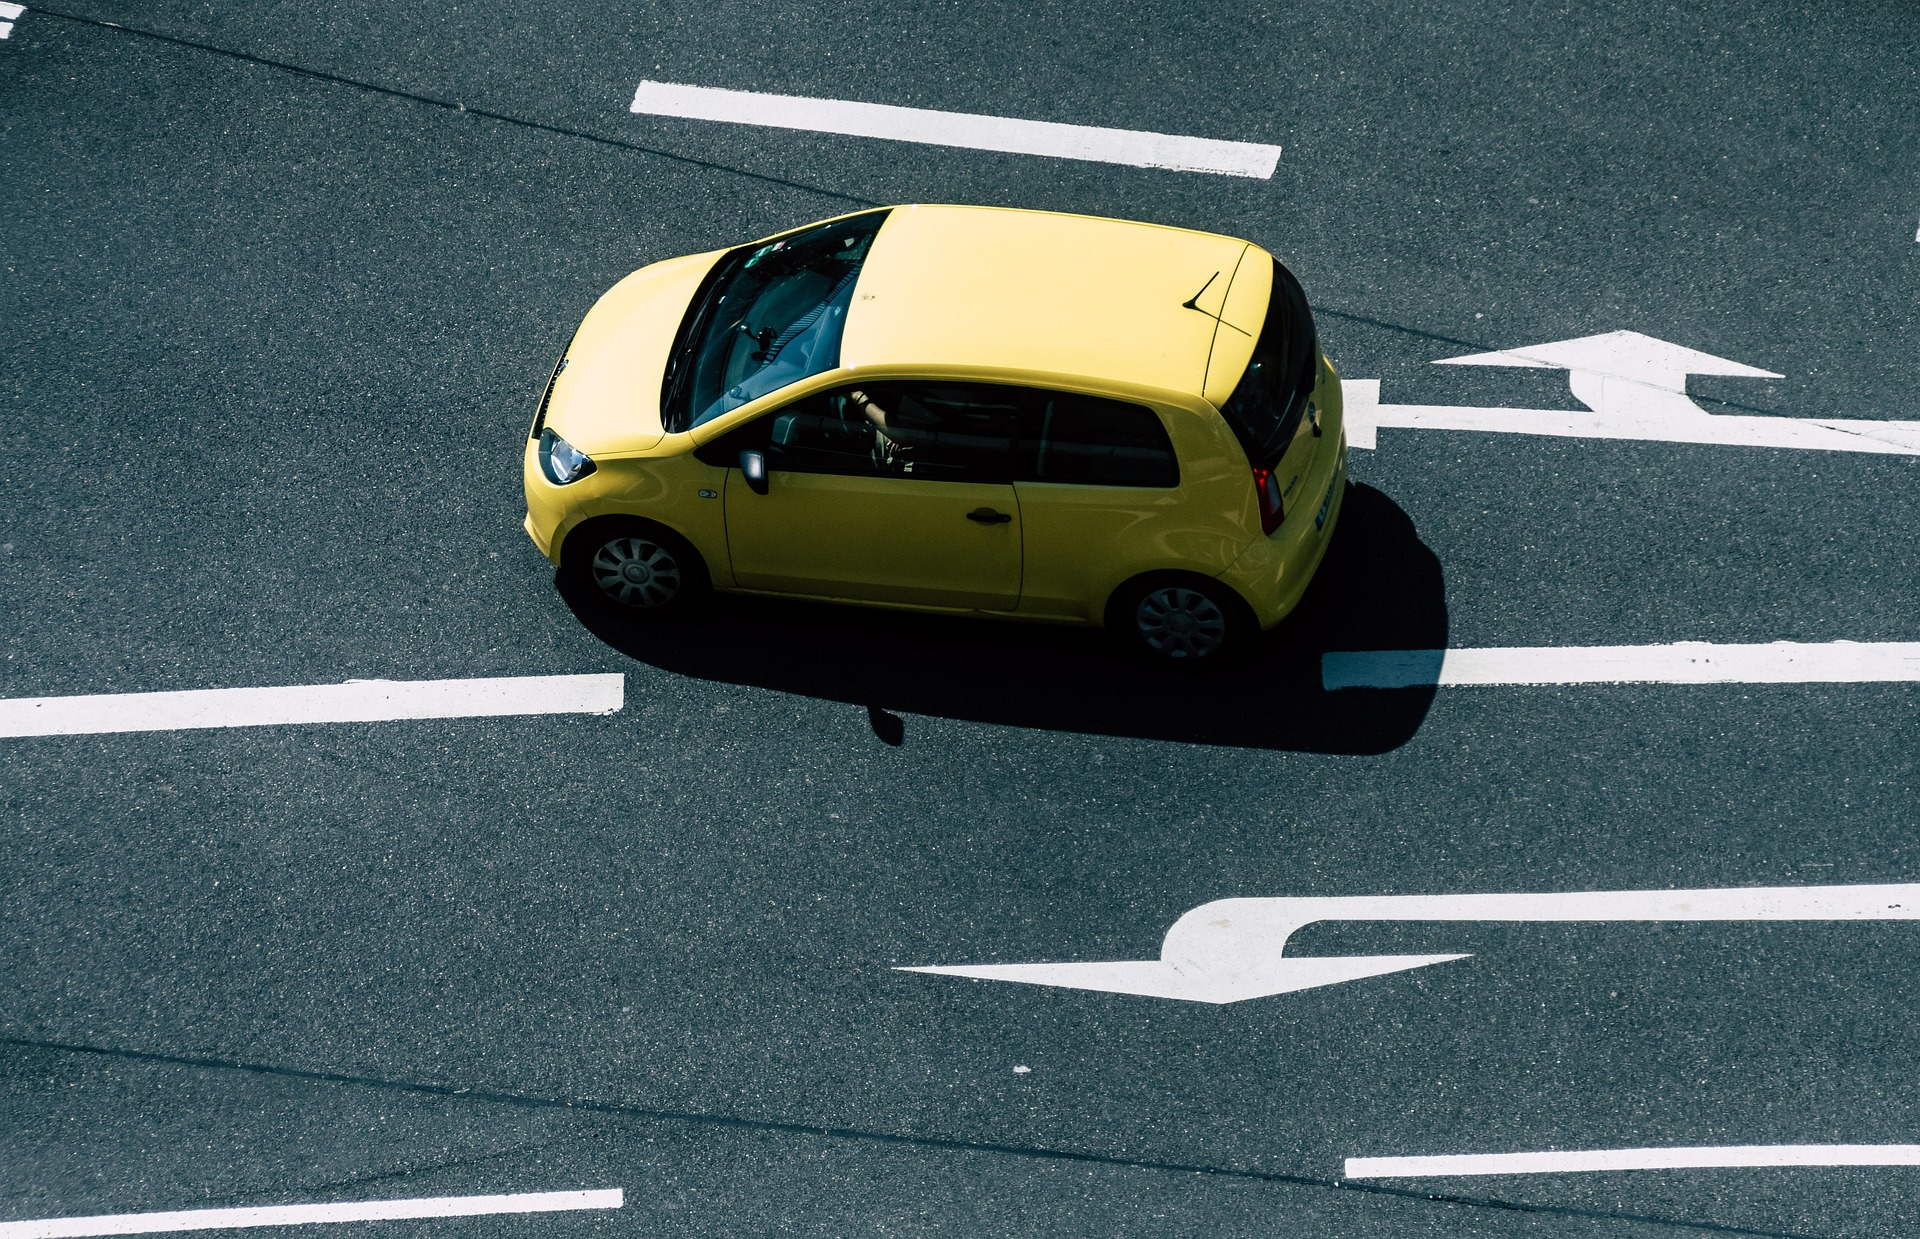
\includegraphics[width=\linewidth,height=0.34\textheight,keepaspectratio]{assets/lane_change_car.jpg}%
      }{%
        
\begin{tikzpicture}
          \node[draw,rounded corners,fill=Panel,minimum width=\linewidth,minimum height=0.34\textheight,align=center,text=Muted]
            {lane-change\\image};
        \end{tikzpicture}%
      }
    \end{column}
    \begin{column}{0.48\textwidth}
      \centering
      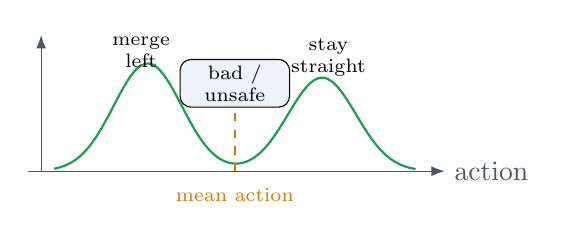
\begin{tikzpicture}[x=0.82cm,y=0.72cm,>=Latex]
        \draw[->,Muted] (-3.2,0) -- (3.25,0) node[right] {action};
        \draw[->,Muted] (-3.0,0) -- (-3.0,2.4);
        \draw[thick,SignalGreen,domain=-2.8:2.8,samples=100]
          plot (\x,{1.9*exp(-1.8*(\x+1.35)^2) + 1.65*exp(-1.8*(\x-1.35)^2)});
        \draw[dashed,thick,WarmGold] (0,0) -- (0,1.15);
        \node[align=center,font=\scriptsize] at (-1.45,2.1) {merge\\left};
        \node[align=center,font=\scriptsize] at (1.45,2.0) {stay\\straight};
        \node[align=center,text=WarmGold,font=\scriptsize] at (0,-0.42) {mean action};
        \node[draw,rounded corners,fill=Panel,text width=1.25cm,align=center,font=\scriptsize,inner sep=2pt] at (0,1.55) {bad / unsafe};
      \end{tikzpicture}
    \end{column}
  \end{columns}

  \vspace{0.28cm}
  \large
  Consider imitation data for self-driving cars:

  \vspace{0.08cm}
  \normalsize
  \begin{itemize}
    \item in similar observed states, driver 1 stays in lane
    \item driver 2 changes lanes
    \item squared-error regression learns the conditional mean action
  \end{itemize}

  \vspace{0.08cm}
  \textbf{Problem:} the mean action can lie between valid modes: a poor command that no expert demonstrated.
  \note{Use the driving image and action-density plot together. The training set can contain two valid behaviors for similar observed states: staying in lane and changing lanes. Squared-error regression treats these as noisy labels around one target and learns the mean. But the mean action may be a poor steering command that no driver demonstrated. This motivates richer policy distributions such as mixtures, autoregressive policies, or diffusion policies later.}
\end{frame}

\begin{frame}{Pitfall 2: Errors Accumulate Over Time}
  \begin{columns}[T,onlytextwidth]
    \begin{column}{0.48\textwidth}
      \centering
      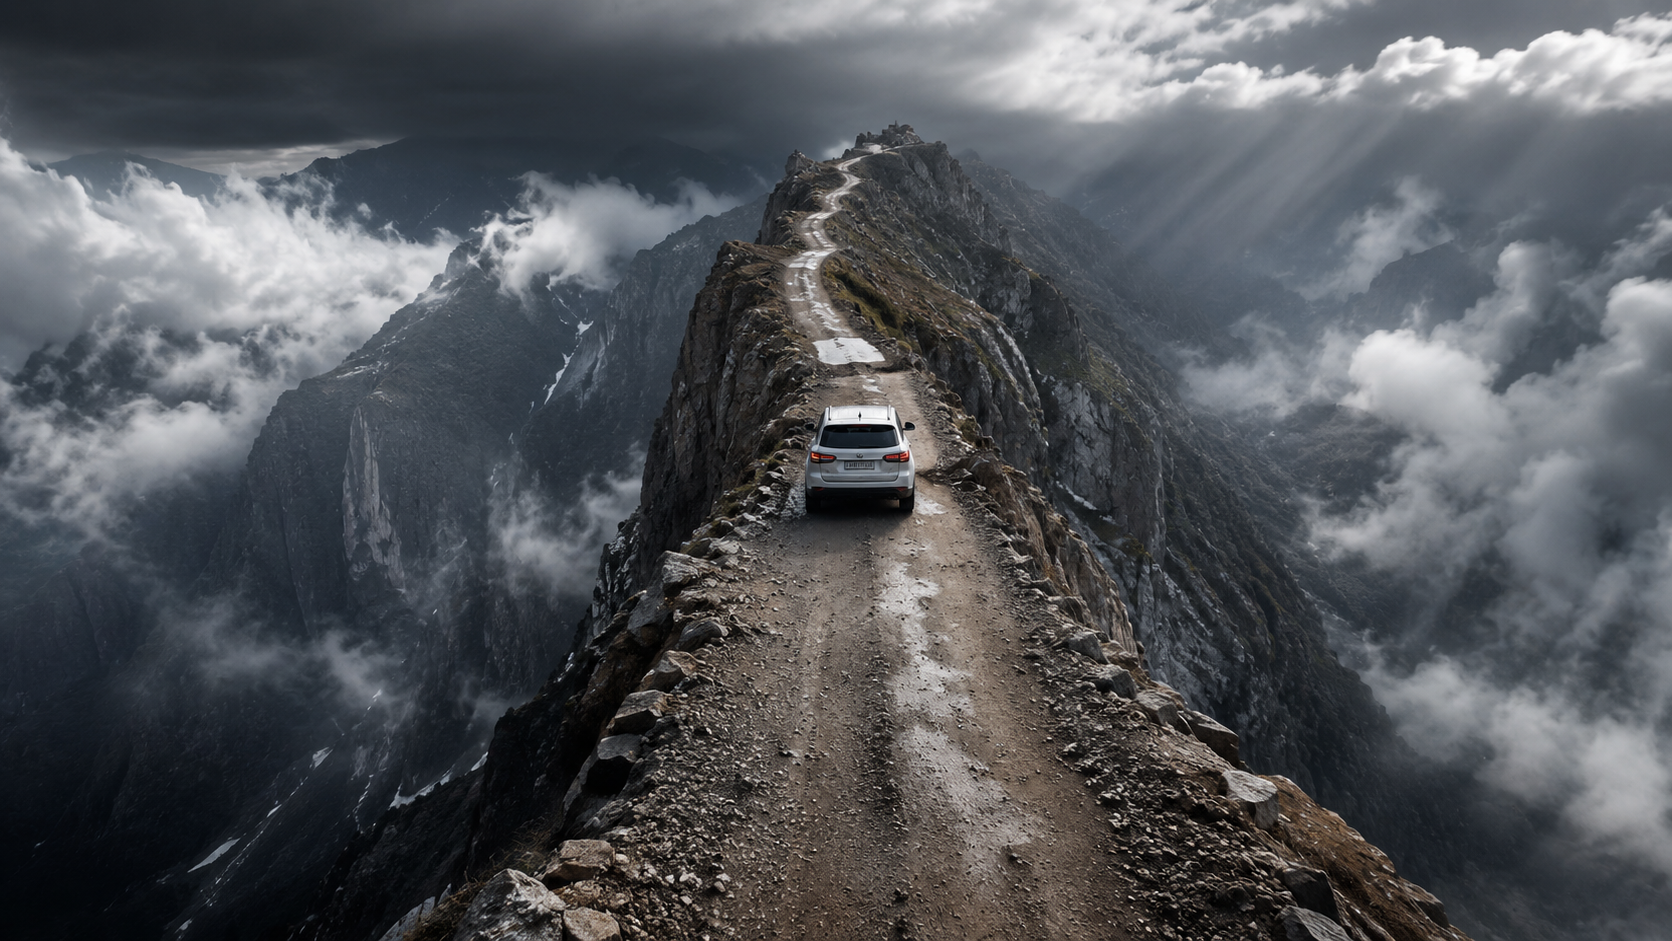
\includegraphics[width=\linewidth,height=0.58\textheight,keepaspectratio]{assets/car-ridge-road.png}
    \end{column}
    \begin{column}{0.48\textwidth}
      \centering
      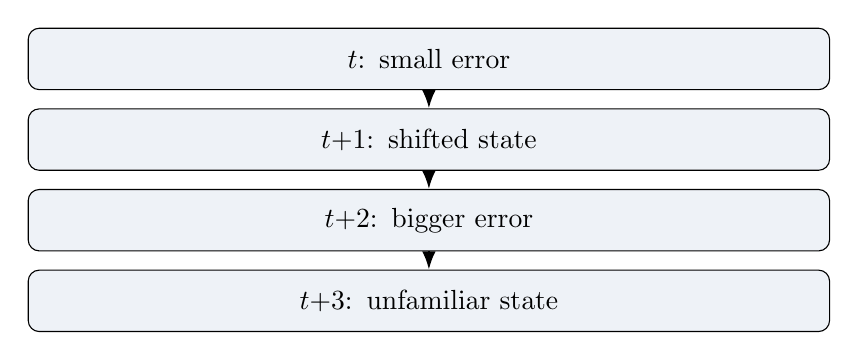
\begin{tikzpicture}[node distance=0.23cm,>=Latex]
        \tikzset{
          driftstep/.style={
            draw,
            rounded corners,
            fill=Panel,
            text width=0.82\linewidth,
            minimum height=0.78cm,
            align=center
          }
        }
        \node[driftstep] (t0) {$t$: small error};
        \node[driftstep,below=of t0] (t1) {$t{+}1$: shifted state};
        \node[driftstep,below=of t1] (t2) {$t{+}2$: bigger error};
        \node[driftstep,below=of t2] (t3) {$t{+}3$: unfamiliar state};
        \draw[->,thick] (t0) -- (t1);
        \draw[->,thick] (t1) -- (t2);
        \draw[->,thick] (t2) -- (t3);
      \end{tikzpicture}
    \end{column}
  \end{columns}

  \vspace{0.24cm}
  \large
  A policy trained only on expert states may not know how to recover from states caused by its own mistakes.

  \vspace{0.12cm}
  \normalsize
  \begin{itemize}
    \item $\rightarrow$ Distribution shift: deployment samples from the learned policy's state distribution, not the expert's.
  \end{itemize}

  \vspace{0.04cm}
  \textbf{Problem:} one-step prediction errors can look small while long rollouts become unstable.
  \note{Use the ridge-road image to make compounding error visceral. Behavior cloning is trained one step at a time on expert states, but deployment is sequential. If the learned policy is slightly off at time t, the next observation may be shifted away from the expert trajectory. The model is then asked to act on a state it was not trained for, which can create an even larger error at the next step. DAgger is the standard intervention-style fix: collect expert labels on states induced by the learned policy.}
\end{frame}

\begin{frame}{Pitfall 3: Imitation Ignores Outcomes}
  \large
  Behavior cloning asks only:

  \vspace{0.12cm}
  \centering
  \Large
  ``What action was taken in this situation?''

  \vspace{0.28cm}
  \raggedright
  \large
  It does not ask:

  \vspace{0.12cm}
  \centering
  \Large
  ``Which action led to the best long-term outcome?''

  \vspace{0.28cm}
  \raggedright
  \normalsize
  Every logged decision becomes a training example.
  The quality of the outcome does not change how strongly it is learned.

  \vspace{0.14cm}
  \textbf{Problem:} behavior cloning reproduces past decisions, but it cannot prefer decisions with better long-term consequences.
  \note{This is the third limitation of imitation learning. Even if the action distribution is expressive and compounding errors are controlled, behavior cloning still has no signal for which logged choices led to better outcomes. It treats the dataset as behavior to reproduce, not evidence for which actions were valuable. This sets up advantage-weighted regression: keep the supervised-learning structure, but weight demonstrations by how good they were.}
\end{frame}

\begin{frame}{The Offline RL Question}
  \Large
  Given logged grain-terminal decisions and delayed outcomes, can we learn a better policy without risky online experimentation?

  \vspace{0.42cm}
  \normalsize
  Logged data:
  \[
    (s_t, a_t, r_t, s_{t+1})
  \]

  \vspace{0.05cm}
  \begin{itemize}
    \item imitation learning asks: what action was likely in the logs?
    \item offline RL asks: which actions led to better long-term outcomes?
  \end{itemize}

  \vspace{0.12cm}
  This talk focuses on offline RL: policy improvement from fixed data.
  \note{Use this as the transition from behavior cloning to offline RL. Behavior cloning predicts the logged operator action. Offline RL uses logged rewards and next states to ask which actions improved long-term outcomes, while avoiding risky online exploration. This is the main focus of the presentation.}
\end{frame}

\begin{frame}{Rewards: Turning Product Outcomes Into a Learning Signal}
  \Large
  A reward turns delayed product outcomes into feedback for decisions:

  \[
    r_t = r(s_t,a_t,s_{t+1})
  \]

  \vspace{0.25cm}
  \normalsize
  For grain loading, rewards can combine:
  \begin{itemize}
    \item train loading progress and throughput
    \item contract quality satisfaction
    \item penalties for rehandling, congestion, and delay
  \end{itemize}

  \vspace{0.2cm}
  Rewards tell the learner what outcomes matter, not just what actions were taken.
  \note{This slide gives the missing bridge from logged outcomes to RL. A reward is a modeling choice: it translates product objectives and operational costs into a scalar signal that can be optimized over time.}
\end{frame}

\section{MDPs and Value Functions}

\begin{frame}{From Value to Action: Learn $Q(s,a)$}
  \Large
  If we know $Q(s,a)$, we can compare actions in the same state.

  \vspace{0.35cm}
  \[
    \text{choose the action with the highest predicted long-term value}
  \]

  \vspace{0.35cm}
  \normalsize
  This is why many RL algorithms learn an action-value function.
  \note{This slide bridges value functions to action selection. V tells us how good a state is; Q tells us which action to take.}
\end{frame}

\begin{frame}{Q-Learning Update}
  \Large
  A one-step target for $Q$:
  \[
    Q(s_t,a_t)
    \leftarrow
    r_t + \gamma \max_{a'} Q(s_{t+1},a')
  \]

  \vspace{0.3cm}
  \normalsize
  Immediate reward plus the best predicted value at the next state.
  \note{Introduce the core Q-learning backup. Do not dwell on stochastic approximation details. The important part is that the max turns value learning into policy improvement.}
\end{frame}

\begin{frame}{Greedy Policy Improvement}
  \Large
  Once we have $Q$, improve the policy by acting greedily:
  \[
    \pi_{\mathrm{new}}(s)
    =
    \arg\max_a Q(s,a)
  \]

  \vspace{0.35cm}
  \normalsize
  This is the basic RL loop:
  \[
    \text{estimate values} \rightarrow \text{choose better actions}.
  \]
  \note{Make the policy improvement idea explicit before discussing why it is dangerous offline.}
\end{frame}

\begin{frame}{Why Q-Learning Is Dangerous Offline}
  \Large
  Offline data only covers some actions.

  \vspace{0.35cm}
  \[
    \max_a Q(s,a)
  \]

  \vspace{0.25cm}
  \normalsize
  The max may select an action the dataset barely supports, where $Q$ is just a guess.

  \vspace{0.25cm}
  \takeaway{The same maximization that improves policies online can exploit value errors offline.}
  \note{This is the teaser for the offline RL section. Later, support mismatch and IQL will make this precise.}
\end{frame}

\section{Idea 2: Conservative Value Learning}

\begin{frame}{Problem: Offline Values Can Be Overconfident}
  \Large
  To compute useful weights, we need value estimates.

  \vspace{0.35cm}
  \normalsize
  But value estimation is harder offline:
  \begin{itemize}
    \item online learning can test actions and correct bad guesses,
    \item offline learning cannot collect new feedback,
    \item unsupported actions may receive overly optimistic predicted values.
  \end{itemize}

  \vspace{0.35cm}
  \begin{block}{Question}
    How can we learn values without trusting predictions where the data is weak?
  \end{block}
  \note{This is the only place to briefly reintroduce why offline value learning is hard. Keep it short.}
\end{frame}

\begin{frame}{Central Idea: Be Pessimistic Where Evidence Is Weak}
  \centering
  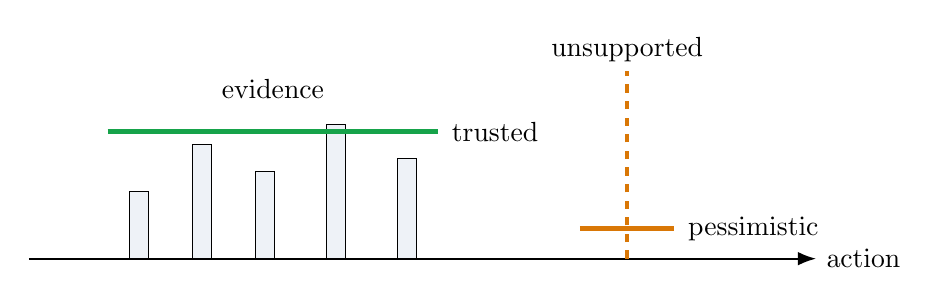
\begin{tikzpicture}[>=Latex,x=1cm,y=0.85cm]
    \draw[->,thick] (0,0) -- (10,0) node[right] {action};
    \foreach \x/\h in {1.4/1.0,2.2/1.7,3.0/1.3,3.9/2.0,4.8/1.5} {
      \draw[fill=Panel] (\x-0.12,0) rectangle (\x+0.12,\h);
    }
    \node[above] at (3.1,2.25) {evidence};
    \draw[SignalGreen,ultra thick] (1.0,1.9) -- (5.2,1.9);
    \node[right] at (5.25,1.9) {trusted};
    \draw[WarmGold,dashed,ultra thick] (7.6,0) -- (7.6,2.8);
    \node[above] at (7.6,2.8) {unsupported};
    \draw[WarmGold,ultra thick] (7.0,0.45) -- (8.2,0.45);
    \node[right] at (8.25,0.45) {pessimistic};
  \end{tikzpicture}

  \vspace{0.35cm}
  \Large
  Conservative value learning lowers confidence away from the logged data.

  \vspace{0.2cm}
  \normalsize
  The policy should not be attracted to actions whose value is high only because the model is guessing.
  \note{This slide conveys the CQL principle visually. Pessimism is a guardrail against unsupported optimism.}
\end{frame}

\begin{frame}{Representative Method: CQL}
  \Large
  Conservative Q-Learning changes the value-learning objective.

  \vspace{0.35cm}
  \normalsize
  Its principle is simple:
  \begin{itemize}
    \item fit observed transitions in the dataset,
    \item penalize high values assigned to actions not well supported by the dataset,
    \item prefer policies whose improvement is backed by evidence.
  \end{itemize}

  \vspace{0.35cm}
  \begin{block}{What to remember}
    Do not trust unsupported actions.
  \end{block}

  \vspace{0.1cm}
  \small
  Representative algorithm: Conservative Q-Learning (CQL).
  \note{Avoid the CQL objective. The audience should remember the pessimism principle, not the optimization details.}
\end{frame}

\begin{frame}{Remaining Problem: Can We Avoid the Risk Entirely?}
  \Large
  CQL makes unsupported actions less attractive.

  \vspace{0.35cm}
  \normalsize
  But it still starts from the same danger:

  \vspace{0.2cm}
  \[
    \text{searching over actions can expose value errors.}
  \]

  \vspace{0.35cm}
  \begin{block}{Next question}
    Can we estimate values without maximizing over unsupported actions at all?
  \end{block}
  \note{This transition motivates IQL. The next idea is not just more pessimism; it avoids the problematic maximization step.}
\end{frame}

\section{Online and Model-Based RL}

\begin{frame}{Online RL Loop}
  \centering
  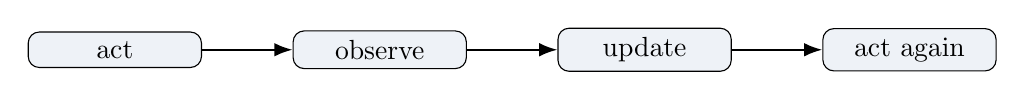
\begin{tikzpicture}[node distance=1.15cm,>=Latex]
    \node[draw,rounded corners,fill=Panel,minimum width=2.2cm] (act) {act};
    \node[draw,rounded corners,fill=Panel,right=of act,minimum width=2.2cm] (obs) {observe};
    \node[draw,rounded corners,fill=Panel,right=of obs,minimum width=2.2cm] (upd) {update};
    \node[draw,rounded corners,fill=Panel,right=of upd,minimum width=2.2cm] (again) {act again};
    \draw[->,thick] (act) -- (obs);
    \draw[->,thick] (obs) -- (upd);
    \draw[->,thick] (upd) -- (again);
  \end{tikzpicture}

  \vspace{0.8cm}
  Online RL learns by interacting while training.
  \note{Keep this short. It exists to set up what offline RL is not.}
\end{frame}

\begin{frame}{Three Common RL Families}
  \centering
  \begin{tabular}{ll}
    \toprule
    \textbf{Family} & \textbf{Basic idea} \\
    \midrule
    Value-based RL & Learn $Q(s,a)$, act greedily \\
    Policy gradient & Directly improve $\pi(a \mid s)$ \\
    Actor-critic & Learn both policy and value \\
    \bottomrule
  \end{tabular}

  \vspace{0.5cm}
  \note{Avoid a DQN/PPO survey. The goal is vocabulary and motivation for critics, actors, and value functions.}
\end{frame}

\begin{frame}{Why Online RL Is Hard in Products}
  \begin{itemize}
    \item Unsafe or costly exploration
    \item Customer-facing experiments
    \item Long feedback delays
    \item Sparse or noisy rewards
    \item Operational constraints and compliance
  \end{itemize}

  \vspace{0.4cm}
  \productbox{When exploration is expensive, risky, or product-constrained, logged data becomes the natural starting point.}
  \note{Give concrete examples: bad recommendations, unsafe robot actions, costly interventions, or agent mistakes.}
\end{frame}

\begin{frame}{Model-Based RL: Learn the Dynamics, Then Plan}
  \[
    \hat{s}_{t+1} = \hat{f}_\theta(s_t,a_t)
  \]

  \[
    a_{0:H}^{\star}
    = \arg\max_{a_{0:H}} \sum_{t=0}^{H} \gamma^t \hat{r}(s_t,a_t)
  \]

  \vspace{0.3cm}
  \takeaway{Model-based RL often looks like MPC with a learned dynamics model.}

  \vspace{0.2cm}
  \small
  Risks: model bias, uncertainty, and compounding rollout error.
  \note{Connect strongly to MPC. Mention that model-based RL can be sample-efficient, but offline rollouts can drift out of distribution.}
\end{frame}

\section{Outlook}

\begin{frame}{What We Could Cover Next}
  This tutorial focused on one branch: model-free Offline RL.

  \vspace{0.25cm}
  Other major directions:
  \begin{itemize}
    \item \textbf{Model-Based RL:} Can we learn a model and plan with it? \\
    World models, imagined rollouts. Examples: Dreamer, TD-MPC, MBPO.

    \vspace{0.16cm}
    \item \textbf{Foundation Models for Robotics:} Can one policy solve many tasks? \\
    Large-scale imitation and vision-language-action models. Examples: RT-1, RT-2, OpenVLA, $\pi_0$.

    \vspace{0.16cm}
    \item \textbf{Sequence Modeling:} Can we replace Bellman updates with sequence modeling? \\
    Trajectories as sequences, Transformer policies. Examples: Decision Transformer, Trajectory Transformer.

    \vspace{0.16cm}
    \item \textbf{Offline-to-Online Adaptation:} How do we keep improving after deployment? \\
    Start from logged data, then fine-tune with limited online interaction.
  \end{itemize}

  \vspace{0.15cm}
  \textbf{Outlook:} Offline RL is increasingly one component of larger data-driven decision-making systems.
  \note{This outlook deliberately points beyond the model-free offline RL branch covered in the tutorial. Keep it conceptual and avoid turning it into a survey.}
\end{frame}

\section{Summary}

\begin{frame}{Summary: Three Ideas, Three Representatives}
  \small
  \centering
  \renewcommand{\arraystretch}{1.25}
  \begin{tabular}{@{}p{0.39\textwidth}p{0.29\textwidth}p{0.19\textwidth}@{}}
    \toprule
    \textbf{Problem} & \textbf{Core idea} & \shortstack[l]{\textbf{Representative}\\\textbf{algorithm}} \\
    \midrule
    Not all demonstrations are equally useful
    & Reweight data
    & AWR \\
    \addlinespace
    Values are unreliable outside the data
    & Conservative value learning
    & CQL \\
    \addlinespace
    Avoid unsupported maximization
    & In-sample value learning
    & IQL \\
    \bottomrule
  \end{tabular}

  \vspace{0.55cm}
  \begin{block}{Main message}
    Modern Offline RL is largely about obtaining reliable value estimates from fixed logged data.
  \end{block}
  \note{End by returning to the three ideas. Mention IDQL only if needed as a complementary policy-representation extension.}
\end{frame}

% Archived: second-half content replaced by the three-idea Offline RL overview.

% Archived: product checklist removed from the shortened conceptual overview.


\begin{frame}{References}
  \tiny
  \nocite{*}
  \bibliographystyle{plain}
  \bibliography{refs}
  \note{Use this slide only if asked for sources. The main talk should cite the relevant papers in place and keep the narrative moving.}
\end{frame}

\end{document}
